% 
\documentclass[10pt,man]{apa6}\usepackage{graphicx, color}
%% maxwidth is the original width if it is less than linewidth
%% otherwise use linewidth (to make sure the graphics do not exceed the margin)
\makeatletter
\def\maxwidth{ %
  \ifdim\Gin@nat@width>\linewidth
    \linewidth
  \else
    \Gin@nat@width
  \fi
}
\makeatother

\usepackage{Sweavel}


\usepackage{microtype}
\usepackage[utf8]{inputenc}
\usepackage[T1]{fontenc}
\usepackage[american]{babel}
\usepackage{csquotes}
\usepackage[style=apa,backend=biber]{biblatex}
\DeclareLanguageMapping{american}{american-apa}
\addbibresource{./data/bibliography.bib}
\usepackage{amsmath}
%\usepackage{mathpazo}
\usepackage{newtxtext}
\usepackage{newtxmath}
\usepackage{siunitx}
\usepackage{listings}
\usepackage[defaultlines=4,all]{nowidow}
\usepackage{placeins}
%\usepackage{courier}
%\usepackage{caption}
%\captionsetup{skip=0pt,labelfont=bf}
\lstset{breaklines=true,showstringspaces=false,basicstyle = \small\ttfamily,}
\newcommand{\Rstat}{\textsf{R}}
\setkeys{Gin}{width=0.8\textwidth}
\usepackage{hyperref}
%\usepackage{booktabs}
%\usepackage[left=1in, right=1in, top=30mm, bottom=30mm, 
      %includefoot, headheight=13.6pt]{geometry} 
      %set margins to be 30mm (needs to include page numbers
\hypersetup{pdfpagelayout=SinglePage} 
% http://www.tug.org/applications/hyperref/ftp/doc/manual.html                                
\hypersetup{
    colorlinks,%
    citecolor=black,%
    filecolor=black,%
    linkcolor=black,%
    urlcolor=black
} % have links but print like standard text 
% http://en.wikibooks.org/wiki/LaTeX/Hyperlinks


\newcommand{\Cases}{\texttt{cases.tsv}}
\newcommand{\Items}{\texttt{items.tsv}}

\usepackage{caption}
\usepackage{minted}













\title{Philippine Science High School-Cordillera Administrative Region University of the Philippines College Admission Test Pre-Test Material: Test Item Analysis and Reliability Analysis Using Classical Test Theory}
\shorttitle{UPCAT Pre-Test Item Analysis}
\author{Joseph S. Tabadero, Jr.}
\affiliation{Science, Mathematics, and Technology Department}
\leftheader{PSHS-CAR Campus}
\abstract{
The University of the Philippines College Admission Test (UPCAT) Pre-test material, which was developed by the Philippine Science High School Main Campus (PSHS-MC), and which has been in use in the Philippine Science High School Cordillera Administrative Region Campus (PSHS-CARC) since the school year 2012-2013, was purported to have high predictive validity with regards to UPCAT results. However, first it is necessary to establish the reliability of the test, as well as the effectiveness of each item in the test to discriminate among high and low performing students.  Therefore, the UPCAT 310-item Pre-Test, given to 78 members of Batch 2014, was subjected to Classical Test Theory test item analysis using R and LibreOffice. The results indicate that the test has good internal consistency, but there is a need to improve several items as well as distractors. Moreover, the results also show that the performance of the students in the pre-test is low.
}
\keywords{item analysis, Classical Test Theory, UPCAT Pre-Test}
\authornote{Joseph S. Tabadero, Jr., Science, Mathematics and Technology Department, Curriculum and Instruction Services Division, Philippine Science High School-Cordillera Administrative Region Campus, Baguio City.

  Correspondence concerning this article should be addressed to Joseph S. Tabadero, Jr., Science, Mathematics and Technology Department, Curriculum and Instruction Services Division, Philippine Science High School-Cordillera Administrative Region Campus, Purok 12, Irisan Lime Kiln, Irisan, Baguio City. Email: josepuses@gmail.com}

\begin{document}
\maketitle
\tableofcontents
\listoftables
\listoflistings
\section{Introduction}

Write some cited related literatures here.

\subsection{Definition of Terms}
The following terms are defined as they are used in this study.

\paragraph{Bad item} This is an item that is too hard, too easy, or has a very low item-total correlations. The rules for determining bad items is summarized in Table~\ref{tab:rule}.

\begin{flushleft}
\captionof{table}{\label{tab:rule} Rules for determining bad items}
\begin{tabular}{ll}
\toprule
Description of item & Rule \\
\midrule
Too hard & mean < 0.1\\
Too easy & mean > 0.9\\
Low r & r < 0.3\\
\bottomrule
\end{tabular}
\end{flushleft}

\section{Methods}
The UPCAT 310-item Pre-Test was administered to 78 members of Batch 2014. The test ran for a total of 3 hours, compared to the 3 hours and 45 minutes in the actual UPCAT. The students' responses were encoded in a spreadsheet file,\Cases, using LibreOffice Calc. \Cases\ was saved in the folder \texttt{data}. The questions, choices and answer key were encoded in the file \Items, which was saved in the folder \texttt{meta}. Choice A was encoded as "1", choice B as "2", choice C as "3", choice D as "4", and choice E as "5". 

The data were imported in R for tests of item-total correlation, index of difficulty, and reliability. These tests were conducted using the \texttt{psych} package. Additionally, the \texttt{CTT} package was used to perform Spearman-Brown prediction. Distractor analysis was then performed using LibreOffice Calc. 

\subsection{Preparation of Data for Data Analysis}

\paragraph{Importing Data} To import the response data to \Rstat{} the researcher used the code in Listing \ref{code:preliminaries}. Listing \ref{code:preliminaries} also set the initial settings, and loaded needed packages and metadata (e.g. the answer key).
\begin{center}
\captionof{listing}{\label{code:preliminaries} \Rstat{} code for initial settings, loading needed packages and metadata.}
\begin{Schunk}
\begin{Sinput}
options(stringsAsFactors = FALSE)
options(width = 80)
library(psych)  # used scoring and alpha
library(CTT)  # used for spearman brown prophecy
cases <- read.delim("data/cases.tsv")
items <- read.delim("meta/items.tsv")
items$variable <- paste("item", items$item, sep = "")
\end{Sinput}
\end{Schunk}

\end{center}

\paragraph{Treatment of missing items} To prepare for test item analysis, the score of each student is computed using Listing \ref{code:scoring}. The \lstinline{missing = FALSE} option tells \Rstat{} not to include missed items as wrong answers.

\begin{center}
\captionof{listing}{\label{code:scoring}The \Rstat{} code for computing the scores of each student}
\begin{Schunk}
\begin{Sinput}
itemstats <- score.multiple.choice(key = items$correct, data = cases[, items$variable], 
    score = TRUE, totals = TRUE, missing = FALSE, short = FALSE)
\end{Sinput}
\end{Schunk}

\end{center}

\subsection{Initial Inspection of Items}

\paragraph{Initial item analysis} Listing \ref{code:computation} lists the item numbers, the correct response (key), the proportion giving the response A(1), B(2), C(3), D(4), and E(5), the item-total correlation (r), the sample size (n), and the proportion correct (mean). The output is shown in Appendix~\ref{output:proportion}.
\begin{center}
\captionof{listing}{\label{code:computation} The \Rstat{} code that shows the item number, correct response (key), the proportion giving response A(1), B(2), C(3), D(4), and E(5), the item-total correlation (r), the sample size (n), and the proportion correct (mean)}
\begin{Schunk}
\begin{Sinput}
results <- itemstats$item.stats[, c("key", "1", "2", "3", "4", "5", "r", "n", "mean")]
\end{Sinput}
\end{Schunk}

\end{center}

\paragraph{Determination of outliers} A stem plot was required by the researcher to determine whether there are outliers in the result. These outliers may be deleted.

\begin{center}
\captionof{listing}{\label{code:stem} \Rstat{} code for computing skewness and kurtosis, and for displaying the stem plot for scores.}
\begin{Schunk}
\begin{Sinput}
scases <- data.frame(score.multiple.choice(key = items$correct, data = cases[, items$variable], 
    score = FALSE))
scases$correct <- apply(scases, 1, mean)
scases$id <- cases$id
description <- psych::describe(scases$correct)
stem(scases$correct)
\end{Sinput}
\begin{Soutput}

  The decimal point is 1 digit(s) to the left of the |

  3 | 9
  4 | 012223444
  4 | 55578
  5 | 12
  5 | 5
\end{Soutput}
\end{Schunk}

\end{center}

\subsection{Reliability}
The internal consistency using Cronbach's alpha was then computed using the code in Listing~\ref{code:cronalpha}.
\begin{center}
\captionof{listing}{\label{code:cronalpha} This \Rstat{} code computes the value of the Cronbach's alpha for the measure of the test's internal consistency.}
\begin{Schunk}
\begin{Sinput}
CronAlpha <- itemstats$alpha
\end{Sinput}
\end{Schunk}

\end{center}

\subsection{Removal of poor items}
It is now necessary to tell \Rstat{} how to flag bad items, including the items that are either too difficult or too easy, and the items with very low item-total correlations, as specified by the rule in Table \ref{tab:rule}.

\begin{center}
\captionof{listing}{\label{code:baditems} The \Rstat{} code setting the rules for determining and displaying the bad items, including very easy and very difficult items, and items with very low item-total correlations.}
\begin{Schunk}
\begin{Sinput}
rules <- list(tooEasy = 0.9, tooHard = 0.1, lowR = 0.15)  # Sets the rules for flagging bad items
itemstats$item.stats$lowR <- itemstats$item.stats$r < rules$lowR
LowR <- row.names(itemstats$item.stats[itemstats$item.stats$lowR, ])  # Displays items with low item-total correlation when LowR is called
itemstats$item.stats$lowR[is.na(itemstats$item.stats$lowR)] <- TRUE
itemstats$item.stats$tooEasy <- itemstats$item.stats$mean > rules$tooEasy
TooEasy <- row.names(itemstats$item.stats[itemstats$item.stats$tooEasy, ])  # Displays too easy items when TooEasy is called
itemstats$item.stats$tooHard <- itemstats$item.stats$mean < rules$tooHard
TooHard <- row.names(itemstats$item.stats[itemstats$item.stats$tooHard, ])  # Displays too hard items when TooHard is called
itemstats$item.stats$baditem <- with(itemstats$item.stats, (lowR | tooHard | tooEasy))
baditems <- row.names(itemstats$item.stats[itemstats$item.stats$baditem, ])  # Displays all of the bad items when baditems is called
\end{Sinput}
\end{Schunk}

\end{center}

Consequently, the good items are coded as the negation of bad items, as shown in Listing~\ref{code:gooditems}. The determination of good items is then used for the computation of predicted number of items using Spearman-Brown prophecy formula for a given Cronbach's alpha of 0.8.
\begin{center}
\captionof{listing}{\label{code:gooditems} \Rstat{} code to determine good items for use in Spearman-Brown prophecy}
\begin{Schunk}
\begin{Sinput}
gooditems <- row.names(itemstats$item.stats[!itemstats$item.stats$baditem, ])  # Defined for computation of Spearman-Brown predicted value for a given Cronbach's alpha
\end{Sinput}
\end{Schunk}

\end{center}

The reliability can then be calculated on the modified scale 
with the items flagged as bad removed. This is done by through the \Rstat{}, as can be seen in the code in Listing~\ref{code:reditem}.
\begin{center}
\captionof{listing}{\label{code:reditem} \Rstat{} code to calculate the reliability on the modified scale with the items flagged as bad removed}
\begin{Schunk}
\begin{Sinput}
reditemstats <- score.multiple.choice(key = items[items$variable %in% gooditems, 
    "correct"], data = cases[, gooditems])
\end{Sinput}
\end{Schunk}

\end{center}

\paragraph{The Spearman Brown estimate} The Spearman Brown prophecy formula provides a means of estimating the number of items required to achieve a given alpha. 

\begin{center}
\captionof{listing}{\label{code:SBF} The \Rstat{} code for estimating the number of items required to achieve a given alpha using the Spearman Brown prophecy formula}
\begin{Schunk}
\begin{Sinput}
sbrown <- list()
sbrown$targetAlpha <- 0.8
sbrown$actualAlpha <- reditemstats$alpha
sbrown$multiple <- CTT::spearman.brown(sbrown$actualAlpha, 0.8, "r")$n.new
sbrown$refinedItemCount <- nrow(reditemstats$item.stats) * sbrown$multiple
sbrown$totalItemCount <- nrow(itemstats$item.stats) * sbrown$multiple
\end{Sinput}
\end{Schunk}

\end{center}

\subsection{Distractor Analysis}

The students' responses and the answer keys were saved in a separate file \texttt{checking.ods} in LibreOffice in order to facilitate distractor. The researcher adapted the distractor analysis procedure in Microsoft Excel, as described in \textcite{elvin}, for LibreOffice. 

\section{Results and Discussion}
\subsection{Initial inspection of items}
The output of the item analysis is shown in Appendix~\ref{output:proportion}. There are no outliers in the scale as shown in the stem plot in Figure~(blahblah). However, the result of the code in Listing~\ref{code:stem}, as shown in Figure~\ref{output:description}, that the scale is positively skewed, indicating that, mostly, the students' scores are below the mean; that is, the students performed poorly in the UPCAT Pre-Test.

\begin{center}
\begin{Schunk}
\begin{Soutput}
  var  n mean   sd median trimmed  mad  min  max range skew kurtosis   se
1   1 18 0.45 0.04   0.44    0.45 0.03 0.39 0.55  0.17 0.82    -0.14 0.01
\end{Soutput}
\end{Schunk}

\captionof{figure}{\label{output:description} Output of Listing~\ref{code:stem}}
\end{center}

\subsection{Reliability}

Using all 310 items the scale has high reliabilty
(alpha = 0.81). (Write discussion of the result of the reliability here.)

\subsection{Removal of poor items}

Overall, the three rules listed in Table~\ref{tab:rule} and coded in Listing~\ref{code:baditems} flagged 
187 of 
310 items as bad. Of these bad items, 0.9 are too easy, 0.1, and 0.15 have low item--total correlation.

\begin{table}[ht]
\caption{\label{lowitem} Item numbers with low item-total correlation per subject area (the same as having a low index of difficulty, meaning, more students with low scores than with high scores were able to get the correct answer).}
\begin{tabular}{lp{0.9\textwidth}}
\toprule
Subject & Item Numbers\\
\midrule
English & 3, 4, 5, 6, 7, 9, 11, 12, 13, 16, 24, 25, 26, 28, 30, 32, 34, 35, 38, 40, 42, 43, 44, 52, 55, 56, 65\\
Filipino & 66, 68, 69, 71, 72, 73, 74, 76, 77, 79, 80, 81, 84, 85, 86, 87, 88, 89, 90, 92, 93, 96, 98, 99, 100, 101, 102, 103, 104, 105, 110, 112, 114, 115, 117, 118, 122, 123, 124\\
Geology & 126, 128, 129, 131, 135, 136, 139, 140, 145, 146, 148, 149, 153, 155, 157, 158\\
Physics & 168, 170, 172, 175, 176, 177, 178, 181, 184, 186, 187, 188, 189\\
Chemistry & 191, 192, 193, 194, 195, 196, 197, 202, 204, 206, 208, 209, 210, 211, 212, 215, 216, 217, 219, 220\\
Biology & 224, 227, 229, 230, 231, 232, 233, 235, 236, 237, 240, 241, 242, 245, 246, 247, 248, 250\\
Math & 251, 253, 254, 255, 258, 259, 261, 262, 263, 265, 266, 268, 269, 272, 273, 275, 276, 277, 279, 280, 282, 284, 286, 287, 288, 290, 291, 292, 295, 297, 298, 299, 300, 301, 303, 304, 305, 306, 307, 308, 309, 310\\
\bottomrule
\end{tabular}
\end{table}

\FloatBarrier
%Item 23 appears to be easy.
%The absence of variability means that item-total correlations 
%can not be calculated for this item.
%A quick look at the item suggests why this might be the case:

%<<inspect_item23>>=
%t(items[items$item == 23, ])
%@





The following figure plots proportion answering the item
correct by item-total correlation.
The horizontal and vertical lines represent rough rules of thumb
 dividing poorer from better items
 (i.e., those with a mean that differentiates
 and an item-total correlation that suggests that the item
 is measuring a meaningful construct).
Thus, items in the middle upper section might be regarded as better items.

However, several caveats should be mentioned.
(a) these are only sample estimates,
(b) what constitutes a good item depends on purpose,
(c) inferences are best made when the external sample is the
 same as the norm sample.


\begin{Schunk}
\begin{Sinput}
plot(r ~ mean, itemstats$item.stats, type = "n")
text(itemstats$item.stats$mean, itemstats$item.stats$r, 1:310)
abline(h = 0.2, v = c(0.5, 0.9))
\end{Sinput}

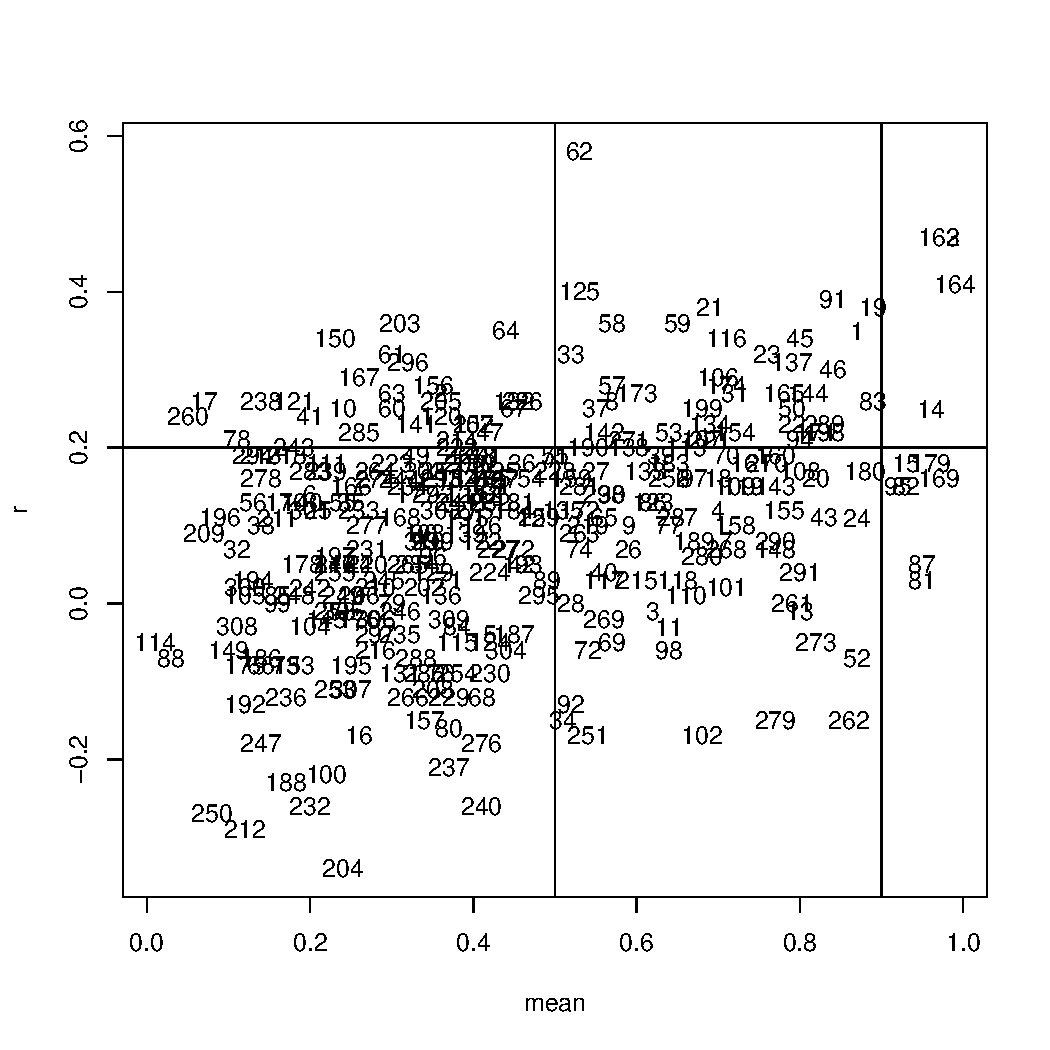
\includegraphics[width=\maxwidth]{figure/listings-plot_mean_by_r} \end{Schunk}





%With the outlier cases the scale reliability was estimated to be 
%itemstats[["alpha"]]
%with the outlier cases removed scale reliability 
%was estimated to be oritemstats[["alpha"]]
%The lesson to be learnt here is that failure to remove outlier
%cases can lead to a gross overestimation of the reliability of a scale.



The resulting reliability was 
0.86 up from
0.81.



The formula suggests  that in order to obtain
an alpha of 0.8,
0.65 times as many items are required.
Thus, the final scale would need around
81 items.
Assuming a similar number of good and bad items,
this would require an initial pool of around
202 items.  
%It should also be noted that these are probably under estimates
%given (a) the relatively small sample size, 
%and (b) item total correlations
%and alpha are likely to be positively biased due to the selection 
%procedure used for identifying good test items. 

\section{Conclusion and Recommendation}
Bad items should be improved through revision. Further work should include distractor analsysis in order to determine whether the choices shold also be revised. Blah blah blah.

\printbibliography

\appendix
\section{\label{output:proportion}Proportion correct and item-total correlations}
\begin{Schunk}
\begin{Sinput}
results
\end{Sinput}
\begin{Soutput}
        key    1    2    3    4    5     r  n mean
item1     4 0.07 0.00 0.04 0.87 0.03  0.35 76 0.87
item2     2 0.01 0.36 0.01 0.01 0.59  0.27 74 0.36
item3     4 0.03 0.01 0.23 0.62 0.11 -0.01 74 0.62
item4     3 0.03 0.05 0.70 0.20 0.03  0.12 76 0.70
item5     5 0.54 0.03 0.00 0.01 0.42 -0.04 76 0.42
item6     4 0.37 0.08 0.34 0.20 0.01  0.14 76 0.20
item7     5 0.01 0.12 0.09 0.07 0.71  0.08 68 0.71
item8     3 0.06 0.10 0.57 0.12 0.15  0.26 68 0.57
item9     1 0.59 0.23 0.03 0.14 0.01  0.10 74 0.59
item10    3 0.09 0.03 0.24 0.16 0.48  0.25 75 0.24
item11    2 0.21 0.64 0.07 0.03 0.05 -0.03 76 0.64
item12    5 0.13 0.24 0.03 0.13 0.47  0.11 76 0.47
item13    1 0.80 0.00 0.01 0.18 0.00 -0.01 76 0.80
item14    3 0.01 0.01 0.96 0.00 0.01  0.25 76 0.96
item15    3 0.00 0.01 0.93 0.00 0.05  0.18 75 0.93
item16    5 0.34 0.09 0.26 0.05 0.26 -0.17 74 0.26
item17    2 0.00 0.07 0.76 0.11 0.07  0.26 76 0.07
item18    1 0.70 0.11 0.01 0.00 0.18  0.16 76 0.70
item19    2 0.04 0.89 0.04 0.01 0.01  0.38 76 0.89
item20    3 0.04 0.12 0.82 0.03 0.00  0.16 76 0.82
item21    1 0.69 0.05 0.03 0.05 0.17  0.38 75 0.69
item22    3 0.16 0.04 0.79 0.01 0.00  0.23 76 0.79
item23    2 0.05 0.76 0.05 0.13 0.00  0.32 76 0.76
item24    1 0.87 0.07 0.00 0.07 0.00  0.11 76 0.87
item25    5 0.03 0.35 0.17 0.24 0.21  0.12 75 0.21
item26    3 0.12 0.04 0.59 0.14 0.11  0.07 74 0.59
item27    2 0.04 0.55 0.03 0.18 0.20  0.17 76 0.55
item28    4 0.05 0.19 0.04 0.52 0.20  0.00 75 0.52
item29    2 0.00 0.42 0.14 0.11 0.33  0.15 76 0.42
item30    1 0.57 0.11 0.24 0.01 0.08  0.14 76 0.57
item31    3 0.03 0.03 0.72 0.01 0.21  0.27 76 0.72
item32    2 0.01 0.11 0.74 0.05 0.09  0.07 76 0.11
item33    2 0.01 0.52 0.07 0.01 0.39  0.32 75 0.52
item34    3 0.12 0.05 0.51 0.12 0.20 -0.15 75 0.51
item35    4 0.11 0.08 0.15 0.25 0.41  0.13 75 0.25
item36    3 0.26 0.01 0.46 0.08 0.18  0.18 76 0.46
item37    4 0.03 0.03 0.25 0.55 0.14  0.25 76 0.55
item38    3 0.03 0.04 0.14 0.30 0.49  0.10 76 0.14
item39    2 0.03 0.63 0.01 0.13 0.20  0.19 76 0.63
item40    2 0.09 0.56 0.04 0.01 0.29  0.04 75 0.56
item41    3 0.19 0.01 0.20 0.12 0.47  0.24 74 0.20
item42    4 0.14 0.00 0.16 0.46 0.24  0.05 76 0.46
item43    2 0.01 0.83 0.01 0.03 0.12  0.11 76 0.83
item44    1 0.26 0.01 0.24 0.07 0.42  0.05 76 0.26
item45    4 0.01 0.00 0.03 0.80 0.16  0.34 76 0.80
item46    2 0.09 0.84 0.03 0.00 0.04  0.30 75 0.84
item47    1 0.42 0.30 0.04 0.24 0.00  0.22 76 0.42
item48    5 0.09 0.33 0.05 0.11 0.41  0.19 75 0.41
item49    3 0.25 0.38 0.33 0.00 0.04  0.19 76 0.33
item50    1 0.79 0.04 0.07 0.04 0.07  0.25 76 0.79
item51    5 0.09 0.17 0.18 0.05 0.50  0.19 76 0.50
item52    5 0.12 0.00 0.00 0.01 0.87 -0.07 76 0.87
item53    3 0.16 0.17 0.64 0.03 0.00  0.22 76 0.64
item54    3 0.32 0.11 0.47 0.07 0.04  0.16 76 0.47
item55    5 0.20 0.32 0.04 0.20 0.24  0.13 75 0.24
item56    1 0.13 0.47 0.31 0.04 0.05  0.13 75 0.13
item57    2 0.05 0.57 0.05 0.15 0.18  0.28 74 0.57
item58    4 0.03 0.05 0.08 0.57 0.27  0.36 74 0.57
item59    3 0.05 0.19 0.65 0.09 0.01  0.36 74 0.65
item60    5 0.04 0.23 0.19 0.23 0.30  0.25 73 0.30
item61    2 0.22 0.30 0.18 0.21 0.10  0.32 73 0.30
item62    5 0.03 0.12 0.08 0.23 0.53  0.58 73 0.53
item63    3 0.06 0.48 0.30 0.11 0.06  0.27 71 0.30
item64    2 0.08 0.44 0.25 0.13 0.10  0.35 71 0.44
item65    4 0.06 0.06 0.17 0.56 0.15  0.11 71 0.56
item66    5 0.75 0.05 0.04 0.01 0.14 -0.08 76 0.14
item67    4 0.08 0.30 0.08 0.45 0.09  0.25 76 0.45
item68    5 0.01 0.30 0.25 0.03 0.41 -0.12 76 0.41
item69    5 0.03 0.00 0.34 0.07 0.57 -0.05 76 0.57
item70    1 0.71 0.00 0.11 0.03 0.16  0.19 76 0.71
item71    5 0.04 0.03 0.36 0.20 0.37  0.03 75 0.37
item72    5 0.09 0.20 0.15 0.01 0.54 -0.06 74 0.54
item73    5 0.00 0.04 0.04 0.75 0.17 -0.08 76 0.17
item74    5 0.36 0.08 0.03 0.00 0.53  0.07 75 0.53
item75    4 0.08 0.05 0.32 0.50 0.05  0.19 76 0.50
item76    3 0.26 0.24 0.36 0.10 0.04 -0.09 72 0.36
item77    3 0.14 0.04 0.64 0.15 0.04  0.10 74 0.64
item78    4 0.04 0.27 0.01 0.11 0.57  0.21 74 0.11
item79    1 0.30 0.09 0.07 0.45 0.09  0.00 74 0.30
item80    2 0.01 0.37 0.05 0.03 0.53 -0.16 75 0.37
item81    3 0.00 0.04 0.95 0.01 0.00  0.03 76 0.95
item82    5 0.05 0.00 0.00 0.01 0.93  0.15 76 0.93
item83    3 0.05 0.03 0.89 0.01 0.01  0.26 76 0.89
item84    4 0.11 0.03 0.08 0.38 0.41 -0.03 76 0.38
item85    3 0.00 0.04 0.16 0.76 0.04  0.01 76 0.16
item86    1 0.62 0.01 0.09 0.26 0.01  0.13 76 0.62
item87    2 0.03 0.95 0.00 0.03 0.00  0.05 76 0.95
item88    3 0.12 0.80 0.03 0.00 0.05 -0.07 75 0.03
item89    3 0.04 0.04 0.49 0.01 0.42  0.03 76 0.49
item90    4 0.08 0.00 0.58 0.34 0.00  0.09 76 0.34
item91    1 0.84 0.13 0.03 0.00 0.00  0.39 76 0.84
item92    2 0.45 0.52 0.00 0.00 0.03 -0.13 75 0.52
item93    3 0.63 0.01 0.34 0.01 0.00  0.08 76 0.34
item94    4 0.13 0.05 0.00 0.80 0.01  0.21 76 0.80
item95    1 0.92 0.07 0.00 0.00 0.01  0.15 76 0.92
item96    1 0.35 0.24 0.15 0.03 0.24  0.06 75 0.35
item97    3 0.04 0.12 0.67 0.13 0.04  0.16 76 0.67
item98    1 0.64 0.01 0.24 0.05 0.05 -0.06 76 0.64
item99    2 0.45 0.16 0.14 0.03 0.23  0.00 74 0.16
item100   2 0.04 0.22 0.72 0.01 0.00 -0.22 76 0.22
item101   4 0.20 0.03 0.07 0.71 0.00  0.02 76 0.71
item102   1 0.68 0.07 0.16 0.05 0.04 -0.17 75 0.68
item103   1 0.34 0.17 0.34 0.05 0.09  0.09 76 0.34
item104   3 0.28 0.08 0.20 0.36 0.07 -0.03 74 0.20
item105   5 0.05 0.31 0.32 0.20 0.12  0.01 75 0.12
item106   3 0.18 0.04 0.70 0.05 0.03  0.29 74 0.70
item107   1 0.68 0.28 0.04 0.00 0.00  0.21 74 0.68
item108   1 0.80 0.08 0.04 0.08 0.00  0.17 74 0.80
item109   2 0.01 0.72 0.03 0.04 0.20  0.15 74 0.72
item110   1 0.66 0.09 0.05 0.18 0.01  0.01 74 0.66
item111   4 0.47 0.08 0.19 0.22 0.04  0.18 73 0.22
item112   4 0.05 0.50 0.04 0.41 0.00  0.14 74 0.41
item113   1 0.66 0.08 0.22 0.03 0.01  0.20 74 0.66
item114   5 0.68 0.07 0.18 0.07 0.01 -0.05 74 0.01
item115   2 0.34 0.38 0.07 0.12 0.09 -0.05 74 0.38
item116   3 0.05 0.04 0.71 0.14 0.05  0.34 73 0.71
item117   3 0.12 0.08 0.56 0.21 0.03  0.03 73 0.56
item118   3 0.07 0.18 0.65 0.07 0.03  0.03 72 0.65
item119   2 0.10 0.73 0.08 0.07 0.03  0.15 73 0.73
item120   3 0.22 0.15 0.36 0.21 0.07  0.24 73 0.36
item121   1 0.18 0.23 0.40 0.19 0.00  0.26 73 0.18
item122   2 0.08 0.41 0.15 0.21 0.15  0.08 73 0.41
item123   4 0.10 0.16 0.10 0.62 0.03  0.13 73 0.62
item124   1 0.42 0.19 0.29 0.08 0.01 -0.05 73 0.42
item125   3 0.10 0.14 0.53 0.19 0.04  0.40 72 0.53
item126   3 0.23 0.10 0.41 0.24 0.01  0.10 78 0.41
item127   1 0.43 0.08 0.17 0.32 0.00  0.16 77 0.43
item128   4 0.08 0.01 0.52 0.39 0.00  0.14 77 0.39
item129   2 0.17 0.35 0.27 0.21 0.00  0.04 77 0.35
item130   2 0.29 0.40 0.19 0.12 0.00  0.18 78 0.40
item131   1 0.31 0.14 0.27 0.28 0.00 -0.09 74 0.31
item132   3 0.22 0.31 0.45 0.01 0.00  0.26 77 0.45
item133   3 0.09 0.09 0.61 0.21 0.00  0.17 77 0.61
item134   2 0.01 0.69 0.21 0.09 0.00  0.23 78 0.69
item135   4 0.12 0.17 0.19 0.51 0.00  0.12 72 0.51
item136   2 0.12 0.36 0.12 0.41 0.00  0.01 76 0.36
item137   3 0.06 0.06 0.79 0.06 0.01  0.31 78 0.79
item138   2 0.23 0.59 0.04 0.13 0.01  0.20 75 0.59
item139   3 0.03 0.15 0.39 0.43 0.00  0.09 74 0.39
item140   4 0.21 0.16 0.40 0.19 0.04  0.13 57 0.19
item141   1 0.33 0.24 0.22 0.22 0.00  0.23 55 0.33
item142   2 0.24 0.56 0.07 0.13 0.00  0.22 55 0.56
item143   1 0.77 0.12 0.05 0.05 0.01  0.15 78 0.77
item144   3 0.12 0.04 0.81 0.03 0.00  0.27 75 0.81
item145   2 0.18 0.22 0.47 0.14 0.00 -0.02 74 0.22
item146   2 0.41 0.23 0.18 0.18 0.00  0.05 78 0.23
item147   4 0.17 0.21 0.21 0.40 0.00  0.16 75 0.40
item148   2 0.17 0.77 0.01 0.05 0.00  0.07 78 0.77
item149   4 0.52 0.25 0.12 0.10 0.01 -0.06 77 0.10
item150   4 0.03 0.22 0.49 0.23 0.03  0.34 77 0.23
item151   4 0.17 0.28 0.13 0.42 0.00  0.15 76 0.42
item152   4 0.49 0.06 0.05 0.40 0.00  0.23 78 0.40
item153   4 0.24 0.35 0.23 0.18 0.00 -0.08 74 0.18
item154   2 0.11 0.72 0.15 0.03 0.00  0.22 75 0.72
item155   4 0.05 0.01 0.16 0.78 0.00  0.12 77 0.78
item156   1 0.35 0.08 0.18 0.37 0.03  0.28 78 0.35
item157   1 0.34 0.17 0.16 0.34 0.00 -0.15 77 0.34
item158   3 0.04 0.06 0.72 0.17 0.01  0.10 78 0.72
item159   2 0.34 0.52 0.03 0.12 0.00  0.16 77 0.52
item160   4 0.06 0.01 0.15 0.77 0.00  0.19 78 0.77
item161   2 0.18 0.74 0.04 0.00 0.04  0.18 78 0.74
item162   2 0.01 0.97 0.01 0.00 0.00  0.47 77 0.97
item163   4 0.00 0.03 0.00 0.97 0.00  0.47 77 0.97
item164   5 0.00 0.00 0.01 0.00 0.99  0.41 77 0.99
item165   1 0.78 0.14 0.03 0.04 0.01  0.27 77 0.78
item166   1 0.25 0.65 0.05 0.03 0.01  0.15 75 0.25
item167   2 0.48 0.26 0.16 0.08 0.01  0.29 73 0.26
item168   1 0.31 0.27 0.14 0.07 0.22  0.11 74 0.31
item169   3 0.01 0.00 0.97 0.01 0.00  0.16 76 0.97
item170   1 0.17 0.11 0.00 0.32 0.41  0.13 76 0.17
item171   5 0.03 0.04 0.03 0.09 0.82  0.22 77 0.82
item172   3 0.10 0.10 0.53 0.24 0.04  0.12 72 0.53
item173   4 0.03 0.33 0.03 0.60 0.01  0.27 75 0.60
item174   5 0.04 0.09 0.10 0.05 0.71  0.28 77 0.71
item175   3 0.04 0.14 0.12 0.08 0.62 -0.08 77 0.12
item176   1 0.26 0.22 0.25 0.22 0.04 -0.02 72 0.26
item177   5 0.16 0.19 0.08 0.23 0.33  0.14 73 0.33
item178   4 0.24 0.55 0.01 0.19 0.01  0.05 75 0.19
item179   1 0.96 0.01 0.01 0.01 0.00  0.18 77 0.96
item180   2 0.05 0.88 0.03 0.00 0.04  0.17 76 0.88
item181   4 0.01 0.09 0.23 0.45 0.21  0.13 77 0.45
item182   4 0.09 0.12 0.38 0.38 0.03  0.16 76 0.38
item183   1 0.64 0.03 0.07 0.25 0.01  0.18 75 0.64
item184   2 0.24 0.45 0.20 0.03 0.08  0.12 74 0.45
item185   1 0.42 0.11 0.21 0.20 0.06  0.16 71 0.42
item186   3 0.07 0.69 0.14 0.09 0.01 -0.07 70 0.14
item187   4 0.17 0.18 0.15 0.45 0.04 -0.04 71 0.45
item188   3 0.17 0.47 0.17 0.09 0.09 -0.23 76 0.17
item189   1 0.67 0.08 0.05 0.08 0.11  0.08 73 0.67
item190   2 0.14 0.54 0.19 0.09 0.04  0.20 74 0.54
item191   2 0.16 0.39 0.32 0.01 0.12  0.11 77 0.39
item192   4 0.24 0.11 0.21 0.12 0.33 -0.13 76 0.12
item193   2 0.11 0.46 0.22 0.19 0.03  0.05 74 0.46
item194   4 0.26 0.32 0.13 0.13 0.16  0.03 77 0.13
item195   3 0.20 0.21 0.25 0.16 0.17 -0.08 75 0.25
item196   2 0.23 0.09 0.04 0.51 0.13  0.11 77 0.09
item197   5 0.15 0.29 0.25 0.08 0.23  0.06 73 0.23
item198   3 0.12 0.01 0.83 0.03 0.01  0.22 75 0.83
item199   2 0.13 0.68 0.09 0.04 0.05  0.25 76 0.68
item200   4 0.08 0.19 0.12 0.39 0.23  0.18 75 0.39
item201   1 0.41 0.11 0.21 0.12 0.15  0.19 75 0.41
item202   1 0.34 0.43 0.08 0.05 0.09  0.02 74 0.34
item203   4 0.10 0.13 0.29 0.31 0.17  0.36 70 0.31
item204   3 0.19 0.29 0.24 0.04 0.24 -0.34 70 0.24
item205   1 0.36 0.36 0.09 0.16 0.03  0.26 75 0.36
item206   4 0.18 0.11 0.37 0.26 0.08  0.01 65 0.26
item207   5 0.19 0.11 0.21 0.08 0.40  0.23 72 0.40
item208   1 0.35 0.22 0.19 0.07 0.17 -0.11 72 0.35
item209   5 0.29 0.22 0.37 0.05 0.07  0.09 73 0.07
item210   2 0.15 0.28 0.17 0.08 0.32  0.02 65 0.28
item211   4 0.49 0.17 0.09 0.16 0.10  0.11 70 0.16
item212   2 0.55 0.12 0.27 0.03 0.03 -0.29 66 0.12
item213   1 0.14 0.18 0.20 0.42 0.06  0.19 65 0.14
item214   2 0.08 0.38 0.24 0.18 0.12  0.21 66 0.38
item215   2 0.04 0.60 0.19 0.13 0.03  0.03 68 0.60
item216   3 0.11 0.25 0.28 0.30 0.06 -0.06 64 0.28
item217   1 0.23 0.11 0.31 0.17 0.17  0.05 64 0.23
item218   4 0.25 0.34 0.17 0.17 0.08  0.19 65 0.17
item219   3 0.12 0.15 0.54 0.14 0.05  0.10 65 0.54
item220   4 0.23 0.23 0.21 0.27 0.06  0.05 62 0.27
item221   2 0.08 0.69 0.06 0.16 0.00  0.21 62 0.69
item222   2 0.19 0.38 0.27 0.08 0.08  0.20 63 0.38
item223   3 0.30 0.25 0.30 0.13 0.03  0.18 61 0.30
item224   2 0.20 0.42 0.24 0.14 0.00  0.04 59 0.42
item225   3 0.07 0.30 0.43 0.15 0.05  0.17 60 0.43
item226   3 0.16 0.16 0.46 0.20 0.02  0.26 61 0.46
item227   3 0.12 0.29 0.43 0.10 0.05  0.07 58 0.43
item228   2 0.25 0.50 0.07 0.12 0.05  0.17 56 0.50
item229   3 0.11 0.22 0.37 0.28 0.02 -0.12 54 0.37
item230   3 0.17 0.28 0.42 0.08 0.06 -0.09 53 0.42
item231   4 0.20 0.24 0.27 0.27 0.02  0.07 55 0.27
item232   3 0.30 0.31 0.20 0.13 0.06 -0.26 54 0.20
item233   1 0.26 0.28 0.19 0.17 0.11  0.12 54 0.26
item234   3 0.15 0.30 0.32 0.15 0.08  0.15 53 0.32
item235   3 0.17 0.35 0.31 0.13 0.04 -0.04 54 0.31
item236   1 0.17 0.36 0.26 0.17 0.04 -0.12 53 0.17
item237   2 0.25 0.37 0.17 0.12 0.10 -0.21 52 0.37
item238   1 0.14 0.22 0.32 0.20 0.12  0.26 50 0.14
item239   3 0.18 0.41 0.22 0.14 0.06  0.17 51 0.22
item240   2 0.12 0.41 0.29 0.14 0.04 -0.26 51 0.41
item241   3 0.10 0.18 0.38 0.12 0.22  0.13 50 0.38
item242   1 0.20 0.33 0.22 0.14 0.10  0.02 49 0.20
item243   4 0.18 0.28 0.28 0.18 0.08  0.20 50 0.18
item244   3 0.21 0.21 0.31 0.17 0.10  0.16 52 0.31
item245   4 0.15 0.31 0.21 0.29 0.04  0.03 52 0.29
item246   2 0.18 0.31 0.20 0.18 0.14 -0.01 51 0.31
item247   5 0.10 0.22 0.34 0.20 0.14 -0.18 50 0.14
item248   4 0.20 0.30 0.28 0.18 0.04  0.01 50 0.18
item249   1 0.24 0.22 0.37 0.10 0.06  0.01 49 0.24
item250   2 0.25 0.08 0.29 0.27 0.10 -0.27 51 0.08
item251   2 0.10 0.54 0.09 0.15 0.12 -0.17 68 0.54
item252   2 0.12 0.64 0.19 0.03 0.03  0.16 74 0.64
item253   5 0.28 0.14 0.27 0.08 0.23 -0.11 71 0.23
item254   1 0.38 0.12 0.14 0.14 0.22 -0.09 72 0.38
item255   1 0.23 0.32 0.25 0.09 0.12  0.04 69 0.23
item256   3 0.18 0.12 0.64 0.07 0.00  0.16 74 0.64
item257   4 0.39 0.01 0.21 0.36 0.03  0.17 76 0.36
item258   5 0.17 0.26 0.16 0.17 0.23 -0.01 69 0.23
item259   4 0.05 0.22 0.19 0.48 0.05  0.11 73 0.48
item260   5 0.77 0.11 0.04 0.03 0.05  0.24 73 0.05
item261   5 0.00 0.12 0.00 0.09 0.79  0.00 77 0.79
item262   4 0.05 0.03 0.03 0.86 0.04 -0.15 77 0.86
item263   1 0.53 0.11 0.11 0.23 0.03  0.09 74 0.53
item264   2 0.13 0.28 0.09 0.07 0.43  0.17 75 0.28
item265   1 0.32 0.13 0.25 0.05 0.25  0.05 76 0.32
item266   2 0.07 0.32 0.30 0.16 0.15 -0.12 73 0.32
item267   2 0.15 0.39 0.11 0.25 0.11  0.19 75 0.39
item268   4 0.04 0.07 0.12 0.71 0.07  0.07 76 0.71
item269   5 0.14 0.23 0.03 0.04 0.56 -0.02 77 0.56
item270   4 0.06 0.03 0.06 0.76 0.09  0.18 78 0.76
item271   3 0.08 0.12 0.59 0.12 0.08  0.21 73 0.59
item272   3 0.25 0.17 0.45 0.09 0.04  0.07 77 0.45
item273   2 0.07 0.82 0.05 0.04 0.03 -0.05 76 0.82
item274   2 0.08 0.28 0.36 0.09 0.18  0.16 74 0.28
item275   3 0.05 0.15 0.40 0.40 0.00  0.12 75 0.40
item276   5 0.04 0.12 0.10 0.33 0.41 -0.18 69 0.41
item277   3 0.17 0.22 0.27 0.32 0.03  0.10 60 0.27
item278   4 0.32 0.21 0.25 0.14 0.10  0.16 73 0.14
item279   2 0.04 0.77 0.07 0.11 0.00 -0.15 70 0.77
item280   1 0.68 0.15 0.08 0.09 0.00  0.06 75 0.68
item281   2 0.11 0.53 0.25 0.10 0.01  0.15 73 0.53
item282   5 0.07 0.22 0.15 0.13 0.42  0.13 67 0.42
item283   5 0.33 0.09 0.11 0.27 0.20  0.17 66 0.20
item284   3 0.07 0.37 0.33 0.07 0.16  0.05 75 0.33
item285   2 0.23 0.26 0.18 0.13 0.20  0.22 61 0.26
item286   3 0.03 0.05 0.34 0.35 0.23 -0.09 74 0.34
item287   3 0.15 0.13 0.65 0.01 0.05  0.11 75 0.65
item288   4 0.16 0.21 0.16 0.33 0.14 -0.07 63 0.33
item289   3 0.03 0.12 0.83 0.03 0.00  0.23 75 0.83
item290   3 0.00 0.07 0.77 0.15 0.01  0.08 75 0.77
item291   5 0.03 0.05 0.07 0.05 0.80  0.04 74 0.80
item292   4 0.33 0.10 0.09 0.35 0.13  0.14 69 0.35
item293   3 0.20 0.27 0.36 0.10 0.07  0.16 70 0.36
item294   5 0.21 0.14 0.30 0.22 0.13  0.19 63 0.13
item295   5 0.04 0.05 0.28 0.15 0.48  0.01 75 0.48
item296   1 0.32 0.25 0.25 0.08 0.10  0.31 63 0.32
item297   1 0.28 0.15 0.09 0.05 0.42 -0.04 74 0.28
item298   3 0.10 0.16 0.56 0.10 0.07  0.14 68 0.56
item299   1 0.35 0.21 0.21 0.15 0.08  0.08 62 0.35
item300   1 0.12 0.29 0.32 0.20 0.06  0.02 65 0.12
item301   5 0.11 0.10 0.33 0.26 0.20  0.12 61 0.20
item302   2 0.29 0.34 0.26 0.10 0.02  0.17 62 0.34
item303   3 0.20 0.27 0.36 0.05 0.12  0.12 59 0.36
item304   3 0.18 0.21 0.44 0.08 0.08 -0.06 61 0.44
item305   4 0.26 0.24 0.19 0.24 0.06 -0.01 62 0.24
item306   2 0.26 0.28 0.26 0.13 0.07 -0.02 61 0.28
item307   2 0.16 0.25 0.39 0.19 0.02 -0.11 57 0.25
item308   1 0.11 0.25 0.40 0.16 0.09 -0.03 57 0.11
item309   4 0.09 0.16 0.32 0.37 0.07 -0.02 57 0.37
item310   5 0.19 0.08 0.29 0.10 0.34  0.08 59 0.34
\end{Soutput}
\end{Schunk}

\end{document}
